\documentclass[12pt,tikz,border=5pt]{article}
\usepackage[margin=1in]{geometry}
\usepackage{graphicx}
\usepackage{geometry}
\usepackage{fancyhdr}
\usepackage[spanish]{babel}
\decimalpoint
\usepackage{subcaption}
\usepackage{setspace}
\usepackage{natbib}   
\usepackage{hyperref}
\usepackage{enumitem}
\usepackage{amsmath}
\usepackage{amssymb} 
\usepackage{amsfonts}
\usepackage{amsthm}
\newtheorem{ejercicio}{Ejercicio}[section]
\newtheorem*{solucion}{Solución}
% 1. Configurar la separación entre el encabezado y el cuerpo
% headheight: altura de la caja del encabezado (fancyhdr recomienda al menos 15pt)
% headsep: separación física entre el encabezado y el texto (aquí ponemos 1.5cm)
\setlength{\headheight}{15pt}
\geometry{headsep=1.5cm}
% Configurar el estilo de página
\pagestyle{fancy}
\fancyhf{} % Limpia los encabezados y pies de página por defecto
\fancyhead[L]{
\includegraphics[width=2.5cm]{figures/logos_enes.png} \quad 
\includegraphics[width=0.98cm]{figures/logo_iimas.png}} % Logo a la derecha
\fancyfoot[C]{\thepage} % Número de página en el centro del pie (opcional)
\renewcommand{\headrulewidth}{0.1pt} % Quita la línea horizontal del encabezado (opcional)
% Forzar el encabezado en la primera página
\fancypagestyle{plain}{%
    \fancyhf{}
    \fancyhead[L]{
\includegraphics[width=4cm]{figures/logos_enes.png} \quad 
\includegraphics[width=1.6cm]{figures/logo_iimas.png}}
    \fancyfoot[C]{\thepage}
    \renewcommand{\headrulewidth}{0pt}
}
\doublespacing

\title{Cálculo Diferencial e Integral \\ Licenciatura en Ingeniería en Computación \\ G1 2027-1}
\author{Nombre Alumno}
\date{\today}

\begin{document}

\maketitle

\section{Sección}
Lorem ipsum dolor sit amet, consectetur adipiscing elit. Maecenas dictum id lectus in faucibus. Nam id libero auctor, interdum sem nec, lacinia erat. Suspendisse quis congue ante. Aliquam urna leo, dictum quis purus vitae, tempus iaculis lorem. Nunc eu dignissim felis, non finibus dolor. Etiam elementum, nulla at bibendum rhoncus, nulla urna molestie eros, quis ultrices velit lacus sit amet magna. Nunc eget nibh non risus pretium maximus\citep{stewart2001calculo}.

\begin{ejercicio}
  Nulla tempus in turpis a pellentesque. Proin et tempus turpis, elementum tincidunt tellus. Integer vel dictum nulla. Phasellus viverra commodo nisl at cursus. Phasellus ut tortor semper, commodo dui et, volutpat justo. Etiam malesuada maximus est, quis tempus velit egestas id \ref{fig:referenciaA}.

  \begin{figure}[h!]
      \begin{center}
          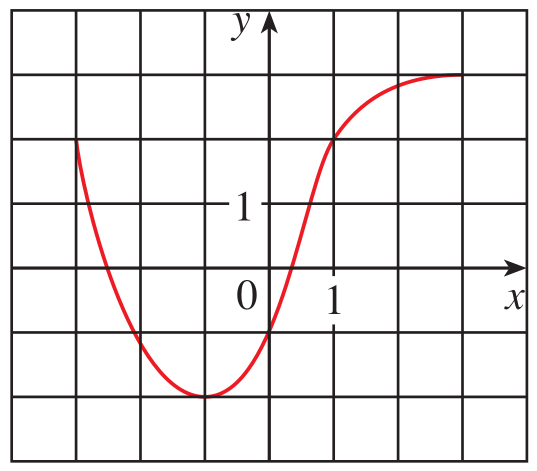
\includegraphics[width=0.30\textwidth]{figures/imagenEjercicio1p1.png}
      \end{center}
      \caption{Gráfica de una función $f$.}\label{fig:referenciaA}
  \end{figure}

  \begin{enumerate}[label=(\alph*)]
    \item Quisque et gravida orci. Integer purus ipsum, aliquam nec dolor vel, tincidunt ultricies metus.
    \item Etiam ornare viverra iaculis. Nullam suscipit dolor sed enim congue faucibus.
    \item Phasellus sed mi mi.
    \item Quisque in nunc quam. Morbi ut nisi eu quam fermentum ultricies.
    \item Nunc eu dignissim felis, non finibus dolor. 
    \item Nullam suscipit dolor sed enim congue faucibus. 
  \end{enumerate}
\end{ejercicio}

\textbf{Sed tincidunt libero sed vestibulum condimentum.} \\
\textit{Phasellus ut tortor semper, commodo dui et, volutpat justo. Etiam malesuada maximus est, quis tempus velit egestas id.}


\begin{ejercicio}
  Nunc vel porta libero. Fusce non ornare dui. Nam eget elit nec elit porta maximus. Nulla tristique tellus et egestas facilisis. Aenean commodo neque a velit luctus, in eleifend est sollicitudin. In in arcu sagittis, iaculis leo porttitor, iaculis eros. Integer non consequat magna. Donec justo odio, aliquam non bibendum vitae, placerat vitae tortor. $$V(r) = \frac{4}{3} \pi r^{3}$$
\end{ejercicio}

\begin{ejercicio}
  Fusce quis dolor ac purus convallis viverra vel sit amet turpis $f(2+h), \, f(x+h), \, \text{ y } \, \frac{f(x+h)-f(x)}{h}$. Quisque aliquam quam ac purus luctus placerat $h\neq0$. 
  \begin{enumerate}[label=(\alph*)]
    \item $f(x) = x - x^{2}$
    \item $f(x) = \frac{x}{x+1}$
  \end{enumerate}
\end{ejercicio}

\begin{ejercicio}
  Nunc erat nisi, pharetra eget quam sed, posuere vehicula felis. Donec vehicula nunc lacus. Fusce aliquet tortor ut mattis placerat. Mauris sagittis eget elit sed aliquet. Fusce efficitur tellus non tortor luctus lacinia. Pellentesque eleifend nec quam non maximus.
  \begin{enumerate}[label=(\alph*)]
    \item $g(x) = \sqrt{x - 5}$
    \item $g(x) = \sqrt[13]{6 - 2x}$
    \item $f(x) = 
      \begin{cases}
        -1, &\text{ si } x \leq -1\\
        3x + 2, &\text{ si } |x| < 1\\
        7 - 2x, &\text{ si } x \geq 1\\
      \end{cases}$
  \end{enumerate}
\end{ejercicio}

\begin{ejercicio}
  Sed gravida tortor in lacus sodales porttitor. Vivamus blandit molestie venenatis. Nam vestibulum eros in tellus tempus imperdiet. Nulla facilisi. In gravida dolor a nulla faucibus, quis lacinia libero blandit. Sed pharetra non diam a cursus. Proin mauris augue, consectetur et interdum eu, iaculis a felis. In dui tellus, cursus quis placerat in, viverra nec nulla. Integer dignissim interdum tellus equation \ref{eq:exp1}.

  \begin{equation}
    \displaystyle\int_{0}^{\pi} \sin{x^2} dx
    \label{eq:exp1}
  \end{equation}
  Aliquam hendrerit interdum metus at cursus. Suspendisse malesuada vulputate ante nec egestas. Sed gravida tortor in lacus sodales porttitor. 
  \begin{equation*}
    \displaystyle\int_{0}^{\pi} \cos{\exp^{x}} dx
    \label{eq:exp2}
  \end{equation*}
\end{ejercicio}
\begin{solucion}
  Ut ultrices lorem mi, eu commodo arcu mollis eu. Pellentesque habitant morbi tristique senectus et netus et malesuada fames ac turpis egestas. Pellentesque ac vestibulum quam. Etiam venenatis vitae dui nec placerat. Suspendisse potenti. Morbi ut eros vel libero cursus vulputate. Quisque cursus facilisis dui, vel volutpat diam feugiat ut. Nam malesuada sed augue eget porttitor. Nunc ut metus accumsan, porta arcu non, gravida lacus. 
  
  \begin{align}
    y &= \tan{x} + \displaystyle\sum_{0}^{N} i^2 \\
    y &= \tan{x} - \displaystyle\frac{3x}{\sqrt[4]{4^{x}}}
  \end{align}
  Quisque vitae eleifend eros.
  \begin{align*}
    y &= \tan{x} + \displaystyle\sum_{0}^{N} i^2 \\
    y &= \tan{x} - \displaystyle\frac{3x}{\sqrt[4]{4^{x}}}
  \end{align*}
  
\end{solucion}

\bibliographystyle{abbrv}
\bibliography{reference}

\end{document}
